\documentclass[11pt,a4paper]{article}

\usepackage[utf8]{inputenc}
\usepackage[T1]{fontenc}
\usepackage[brazil]{babel}
\usepackage[margin=2.5cm]{geometry}
\usepackage{graphicx}
\usepackage{float}
\usepackage{booktabs}
\usepackage{tabularx}
\usepackage{amsmath}
\usepackage{hyperref}
\usepackage{xcolor}
\usepackage{caption}
\usepackage{subcaption}
\usepackage{url}
\usepackage{cite}

\hypersetup{
    colorlinks=true,
    linkcolor=blue!60!black,
    citecolor=blue!60!black,
    urlcolor=blue!60!black
}

\title{\textbf{Classificação Automatizada de Doenças em Folhas de Café Robusta em Condições Reais de Cultivo: Definição do Problema e Análise Exploratória do Dataset RoCoLe}}

\author{
  Natalia Salete Rodrigues \\
  \small Programa de Pós-Graduação em Engenharia Elétrica (PPGEELT) \\
  \small Universidade Federal de Uberlândia (UFU) \\
  \small \href{mailto:natsalete@ufu.br}{\texttt{natsalete@ufu.br}} \\[4pt]
  \small \textit{Disciplina:} Aprendizado de Máquina \\
  \small \textit{Docente:} Prof\textsuperscript{a}. Dr\textsuperscript{a}. Danielli A. Lima
}

\date{\small Etapa 01 do Trabalho de Conclusão de Disciplina --- \today}

\begin{document}

\maketitle

\begin{abstract}
\noindent Apresento, neste relatório, a primeira etapa do meu Trabalho de Conclusão da Disciplina de Aprendizado de Máquina, com foco na definição do problema e na análise exploratória de dados. O objeto de estudo é o \textit{dataset} RoCoLe (Robusta Coffee Leaf), composto por 1.560 imagens de folhas de café robusta capturadas em condições reais de cultivo e distribuídas em seis classes (uma saudável e cinco patológicas). Como estratégia metodológica de integração com as demais atividades do TCD --- nas quais utilizo a ferramenta KNIME ---, converti as imagens em uma representação tabular com 26 \textit{features} numéricas, incluindo estatísticas de cor em RGB/HSV, descritores de textura GLCM, proporções de faixas cromáticas típicas de patologias foliares e métricas de qualidade de imagem. Minha análise exploratória revelou desbalanceamento multiclasse severo (razão de 26,4 vezes entre a classe mais e a menos frequente), alta variabilidade nas condições de aquisição (resoluções entre $720{\times}1280$ e $2322{\times}4128$) e indícios de viés sistemático na captura das imagens, caracterizando os principais desafios para a modelagem preditiva. Esta investigação se alinha diretamente à minha proposta de dissertação de mestrado, que tem como objetivo desenvolver uma arquitetura de \textit{deep learning} com módulos de atenção adaptados para operar sobre este mesmo \textit{dataset}.
\end{abstract}

\vspace{0.5em}
\noindent\textbf{Palavras-chave:} Aprendizado de Máquina; Visão Computacional; Cafeicultura; Análise Exploratória de Dados; Dataset RoCoLe.

\section{Questão de Pesquisa}

Formulo a seguinte questão central para esta investigação:

\begin{quote}
\textit{É possível discriminar automaticamente entre folhas saudáveis e folhas afetadas por diferentes patologias foliares (ferrugem em quatro níveis de severidade e ácaro-vermelho) em imagens de café robusta capturadas em condições reais de cultivo, utilizando uma representação tabular compacta derivada de estatísticas de cor, textura e qualidade de imagem, de modo a estabelecer uma linha de base classificatória robusta para confronto futuro com arquiteturas de \textit{deep learning}?}
\end{quote}

A pergunta apresenta duas dimensões complementares: uma \textit{binária} --- distinguir folhas saudáveis de folhas doentes --- e uma \textit{multiclasse} --- identificar a patologia específica entre cinco categorias distintas. Os resultados reportados na literatura para o \textit{dataset} RoCoLe indicam uma diferença acentuada entre essas tarefas: Santos et al.~\cite{santos2023} alcançaram 95,19\,\% de acurácia na classificação binária com arquitetura ResNet, mas apenas 78,03\,\% na classificação multiclasse, evidenciando que a segunda tarefa permanece aberta a contribuições metodológicas.

\section{Justificativa e Motivação}

\subsection*{Relevância do tema}

A cafeicultura é um dos pilares do agronegócio brasileiro; o Brasil responde por aproximadamente 37\,\% da produção mundial de café~\cite{conab}. Contudo, doenças foliares como a ferrugem (\textit{Hemileia vastatrix}), a cercosporiose (\textit{Cercospora coffeicola}) e a infestação por ácaro-vermelho (\textit{Oligonychus ilicis}) podem comprometer até 30\,\% da safra quando não identificadas precocemente~\cite{matiello2016}. O diagnóstico visual tradicional depende de conhecimento técnico especializado, é subjetivo e sujeito a erros de interpretação, especialmente nos estágios iniciais, quando os sintomas ainda são sutis~\cite{barbedo2018}.

\subsection*{O ambiente dos dados}

O \textit{dataset} RoCoLe~\cite{parraga2019} preenche uma lacuna relevante ao disponibilizar publicamente 1.560 imagens de folhas de café robusta capturadas \textit{in situ}, com fundos complexos, variações naturais de iluminação e presença de outros elementos da cena (solo, galhos, outras folhas). Essa característica contrasta com \textit{datasets} clássicos de fitopatologia como o PlantVillage, compostos por imagens em laboratório com fundo uniforme --- cenário que historicamente infla a acurácia reportada, mas limita a transferibilidade dos modelos para o campo~\cite{barbedo2019}.

\subsection*{Aplicabilidade prática}

Acredito que o desenvolvimento de um \textit{pipeline} capaz de operar sobre imagens de campo pode democratizar o acesso ao diagnóstico fitopatológico especializado, com potencial de impacto relevante para pequenos e médios produtores, que concentram parcela significativa da produção nacional.

\section{Vínculo Acadêmico}

Ingressei em 2026 no Mestrado do Programa de Pós-Graduação em Engenharia Elétrica da UFU (PPGEELT), na linha de pesquisa \textit{Metodologias e Técnicas da Computação}, com projeto de dissertação intitulado \textbf{\guillemotleft{}Classificação Automatizada de Doenças em Folhas de Café usando \textit{Deep Learning} em Condições Reais de Cultivo\guillemotright{}}. Meu plano de pesquisa, de duração de 24 meses, prevê sete etapas metodológicas, entre as quais a \textbf{Etapa 2 --- Preparação e Análise Exploratória do Dataset} coincide diretamente com o escopo da presente atividade.

Dessa forma, este TCD cumpre um duplo papel para mim:
\begin{enumerate}
  \item \textbf{Avanço da Etapa 2 do meu cronograma de mestrado}, produzindo a caracterização quantitativa do \textit{dataset} RoCoLe que pretendo reutilizar na dissertação.
  \item \textbf{Estabelecimento de uma linha de base tabular com classificadores clássicos}, que mais à frente na dissertação confrontarei com a arquitetura baseada em redes neurais convolucionais com módulos de atenção multi-escala que proponho --- fortalecendo a justificativa para o uso de \textit{deep learning} ao demonstrar, quantitativamente, os limites da abordagem clássica.
\end{enumerate}

Minha decisão de representar as imagens como \textit{features} tabulares foi motivada pela escolha do KNIME como ferramenta principal para as etapas subsequentes do TCD. Optei pelo KNIME por concentrar, em um único ambiente, todos os elementos exigidos pelo trabalho --- classificação supervisionada (\textit{Decision Tree}, \textit{Random Forest}, SVM), avaliação de desempenho e visualização ---, dispensando a integração de múltiplas ferramentas. Vale notar que a disciplina apenas \textit{recomenda} o uso de KNIME, Weka ou Python, cabendo à discente a escolha do instrumental mais adequado.

\section{Caracterização dos Dados}

\subsection{Origem e estrutura do \textit{dataset}}

Obtive o RoCoLe a partir do Mendeley Data~\cite{parraga2019}. O \textit{dataset} compreende 1.560 imagens em formato JPEG, acompanhadas de arquivos de anotação em múltiplos formatos (CSV, JSON, COCO, Pascal VOC, XLSX). A planilha \texttt{RoCoLe-classes.xlsx} associa cada arquivo a dois rótulos: um binário (\textit{healthy}/\textit{unhealthy}) e um multiclasse com seis níveis.

\subsection{Pipeline de preparação}

Para alinhamento com as ferramentas da disciplina, desenvolvi um \textit{script} Python de extração de \textit{features} numéricas a partir de cada imagem, gerando o arquivo tabular \texttt{rocole\_features.csv} com 1.560 instâncias ($n$) e 26 atributos preditivos ($m$) mais dois rótulos. A Tabela~\ref{tab:features} descreve os grupos de \textit{features}.

\begin{table}[H]
\centering
\caption{Grupos de \textit{features} tabulares derivadas das imagens do RoCoLe.}
\label{tab:features}
\small
\renewcommand{\arraystretch}{1.15}
\begin{tabularx}{\textwidth}{@{}l X l@{}}
\toprule
\textbf{Grupo} & \textbf{Features} & \textbf{Tipo} \\
\midrule
Cor RGB & \texttt{r\_mean}, \texttt{g\_mean}, \texttt{b\_mean}, \texttt{r\_std}, \texttt{g\_std}, \texttt{b\_std} & Num.\ contínuo \\
Cor HSV & \texttt{h\_mean}, \texttt{s\_mean}, \texttt{v\_mean}, \texttt{h\_std}, \texttt{s\_std}, \texttt{v\_std} & Num.\ contínuo \\
Proporções cromáticas & \texttt{ratio\_healthy\_green}, \texttt{ratio\_rust\_brown\_orange}, \texttt{ratio\_dark\_necrotic} & Num.\ [0,1] \\
Textura GLCM & \texttt{glcm\_contrast}, \texttt{glcm\_homogeneity}, \texttt{glcm\_energy}, \texttt{glcm\_correlation}, \texttt{glcm\_dissimilarity}, \texttt{glcm\_asm} & Num.\ contínuo \\
Dimensões & \texttt{width}, \texttt{height}, \texttt{aspect\_ratio} & Num.\ discreto \\
Qualidade & \texttt{brightness}, \texttt{laplacian\_var} & Num.\ contínuo \\
\midrule
Rótulo binário & \texttt{binary\_label} $\in$ \{healthy, unhealthy\} & Categórico \\
Rótulo multiclasse & \texttt{multiclass\_label} $\in$ \{6 classes\} & Categórico \\
\bottomrule
\end{tabularx}
\end{table}

Computei os descritores de textura GLCM (\textit{Gray Level Co-occurrence Matrix}) em escala de cinza quantizada em 32 níveis, com distância 1 e orientações $\{0, \pi/4, \pi/2, 3\pi/4\}$, seguindo a formulação clássica de Haralick~\cite{haralick1973}. As proporções cromáticas capturam a fração de \textit{pixels} dentro de faixas HSV tipicamente associadas à folha saudável (verde), à ferrugem (marrom/laranja) e a necroses (escuro). Utilizei a variância do Laplaciano como \textit{proxy} de nitidez.

\section{Análise Exploratória de Dados (AED)}

\subsection{Distribuição das classes}

A Figura~\ref{fig:classes} apresenta a distribuição das instâncias nas duas granularidades de rotulação. Na visão binária, observo um \textit{dataset} \textit{quase balanceado}: 791 instâncias saudáveis (50,7\,\%) contra 769 doentes (49,3\,\%). Na visão multiclasse, entretanto, o cenário se inverte radicalmente: a classe majoritária (\textit{healthy}, 791) é 26,4 vezes maior que a minoritária (\textit{rust\_level\_4}, 30 instâncias). As classes de ferrugem apresentam decaimento monotônico com a severidade --- \textit{rust\_level\_1}: 344, \textit{rust\_level\_2}: 166, \textit{rust\_level\_3}: 62, \textit{rust\_level\_4}: 30 ---, refletindo a raridade natural de lesões severas no campo.

\begin{figure}[H]
\centering
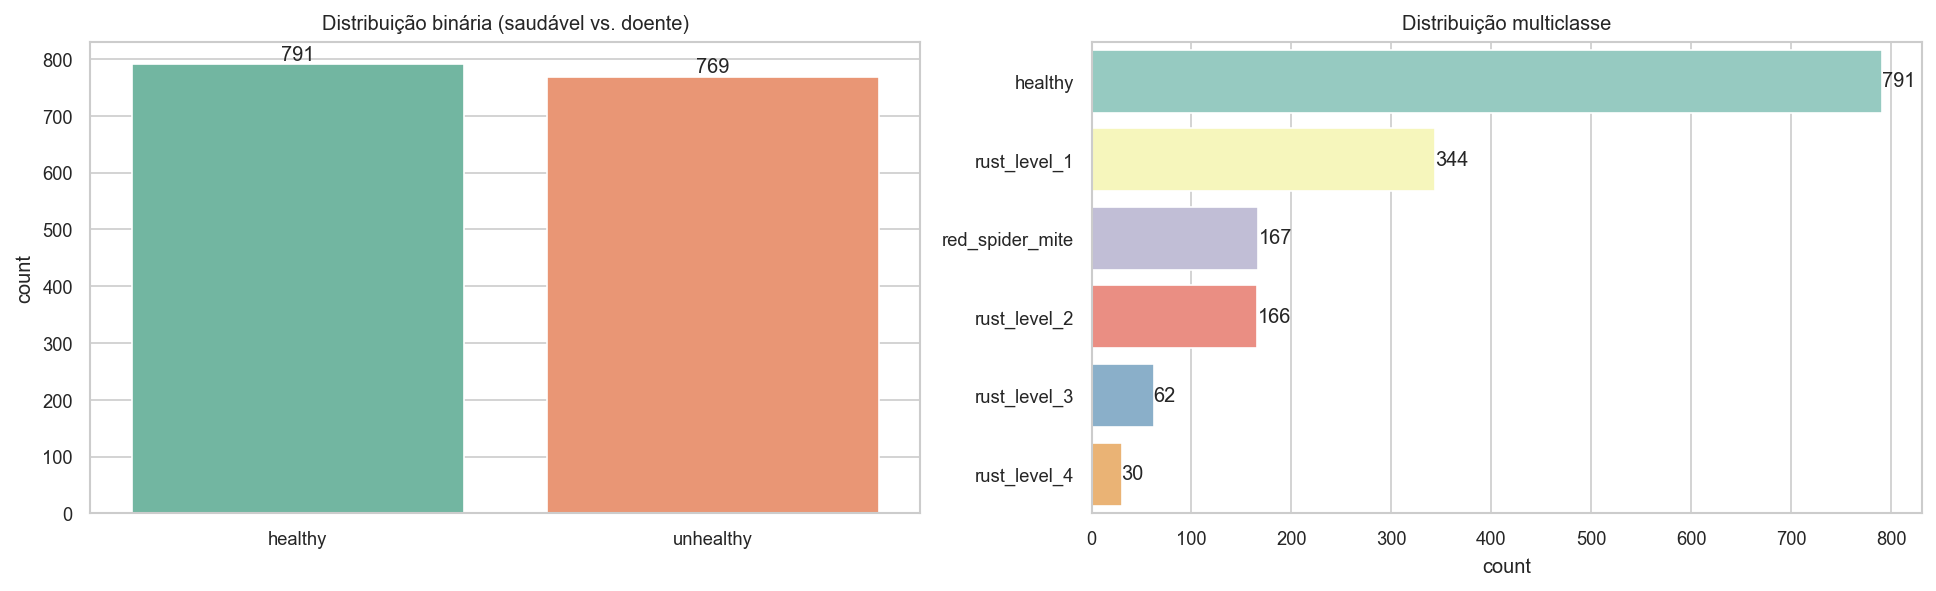
\includegraphics[width=0.95\textwidth]{class_distribution.png}
\caption{Distribuição das instâncias nas visões binária (esquerda) e multiclasse (direita) do \textit{dataset} RoCoLe.}
\label{fig:classes}
\end{figure}

Avalio que esse desbalanceamento é, possivelmente, a principal fonte da queda de desempenho na classificação multiclasse reportada por Santos et al.~\cite{santos2023} (78,03\,\%) em relação à binária (95,19\,\%). Caracterizá-lo quantitativamente é um passo fundamental para conduzir adequadamente quaisquer experimentos subsequentes de modelagem.

\subsection{Qualidade e variabilidade de aquisição}

A Figura~\ref{fig:quality} evidencia a alta variabilidade das condições de captura, característica que diferencia o RoCoLe de \textit{datasets} em ambiente controlado. As dimensões variam de $720{\times}1280$ a $2322{\times}4128$ \textit{pixels}, o brilho médio oscila entre $\mu=116{,}3$ e desvio $\sigma=13{,}9$, e a variância do Laplaciano (\textit{proxy} de nitidez) abrange duas ordens de grandeza (mediana de 752,8, com extremos entre 109,8 e 12.363,9). Essa heterogeneidade reflete diretamente as condições reais de cultivo, em que diferentes dispositivos, ângulos e iluminações naturais foram empregados na captura.

\begin{figure}[H]
\centering
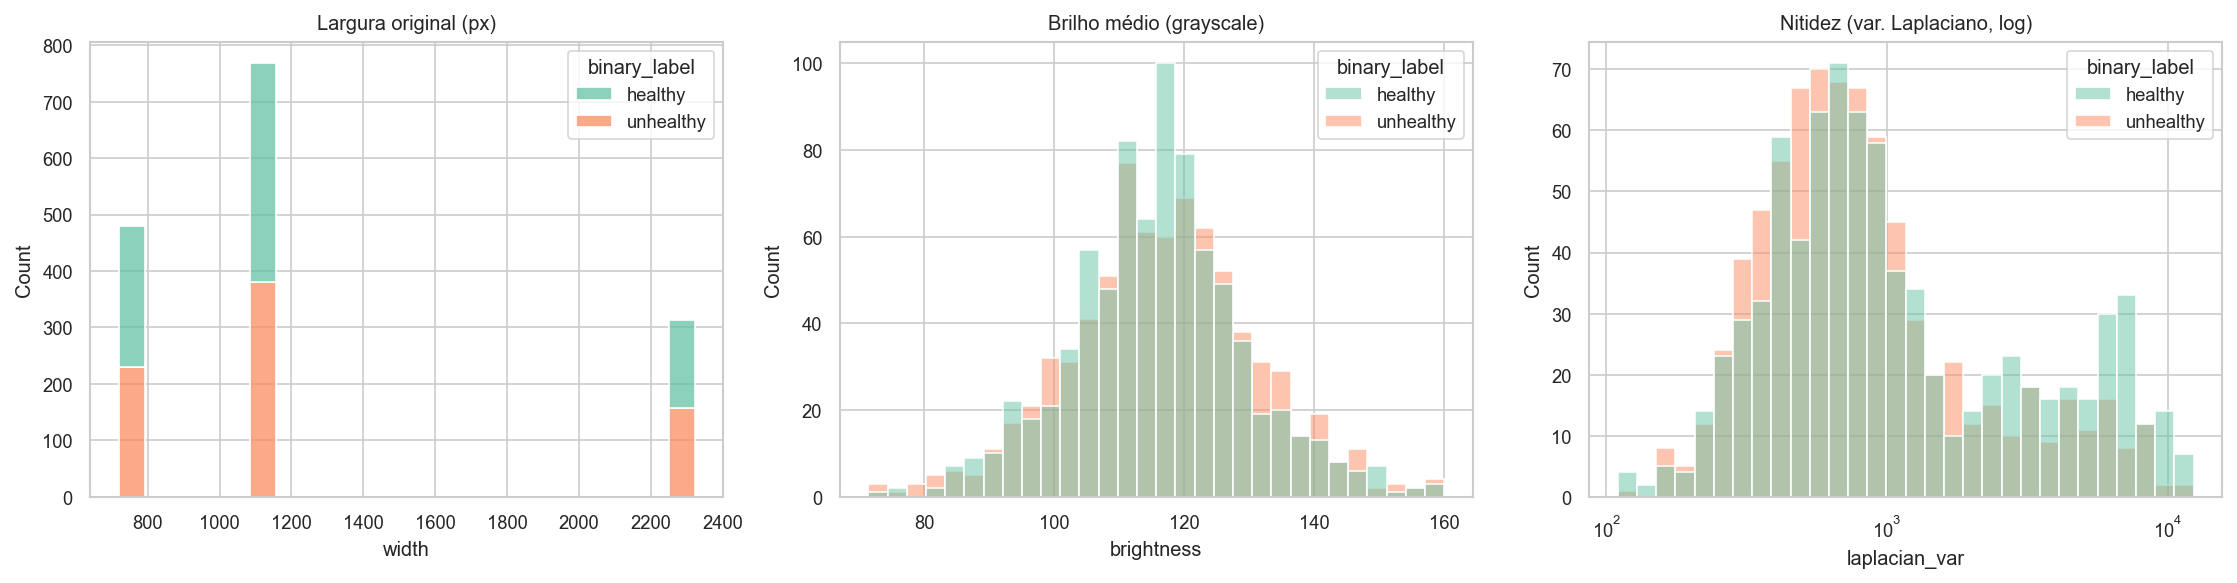
\includegraphics[width=0.95\textwidth]{image_quality.png}
\caption{Distribuição das características de aquisição: largura original, brilho médio e variância do Laplaciano (escala logarítmica).}
\label{fig:quality}
\end{figure}

\subsection{Distribuição das \textit{features} de cor por classe}

A Figura~\ref{fig:histcolor} apresenta os histogramas sobrepostos das seis \textit{features} médias de cor (RGB e HSV) estratificadas pela rotulação binária. Observo sobreposição substancial entre as distribuições de folhas saudáveis e doentes --- especialmente em \texttt{r\_mean} e \texttt{v\_mean} ---, indicando que nenhuma \textit{feature} de cor isolada é suficiente para separar as classes. Esse achado reforça a necessidade de modelos capazes de combinar múltiplas \textit{features} não linearmente (como árvores e \textit{ensembles}).

\begin{figure}[H]
\centering
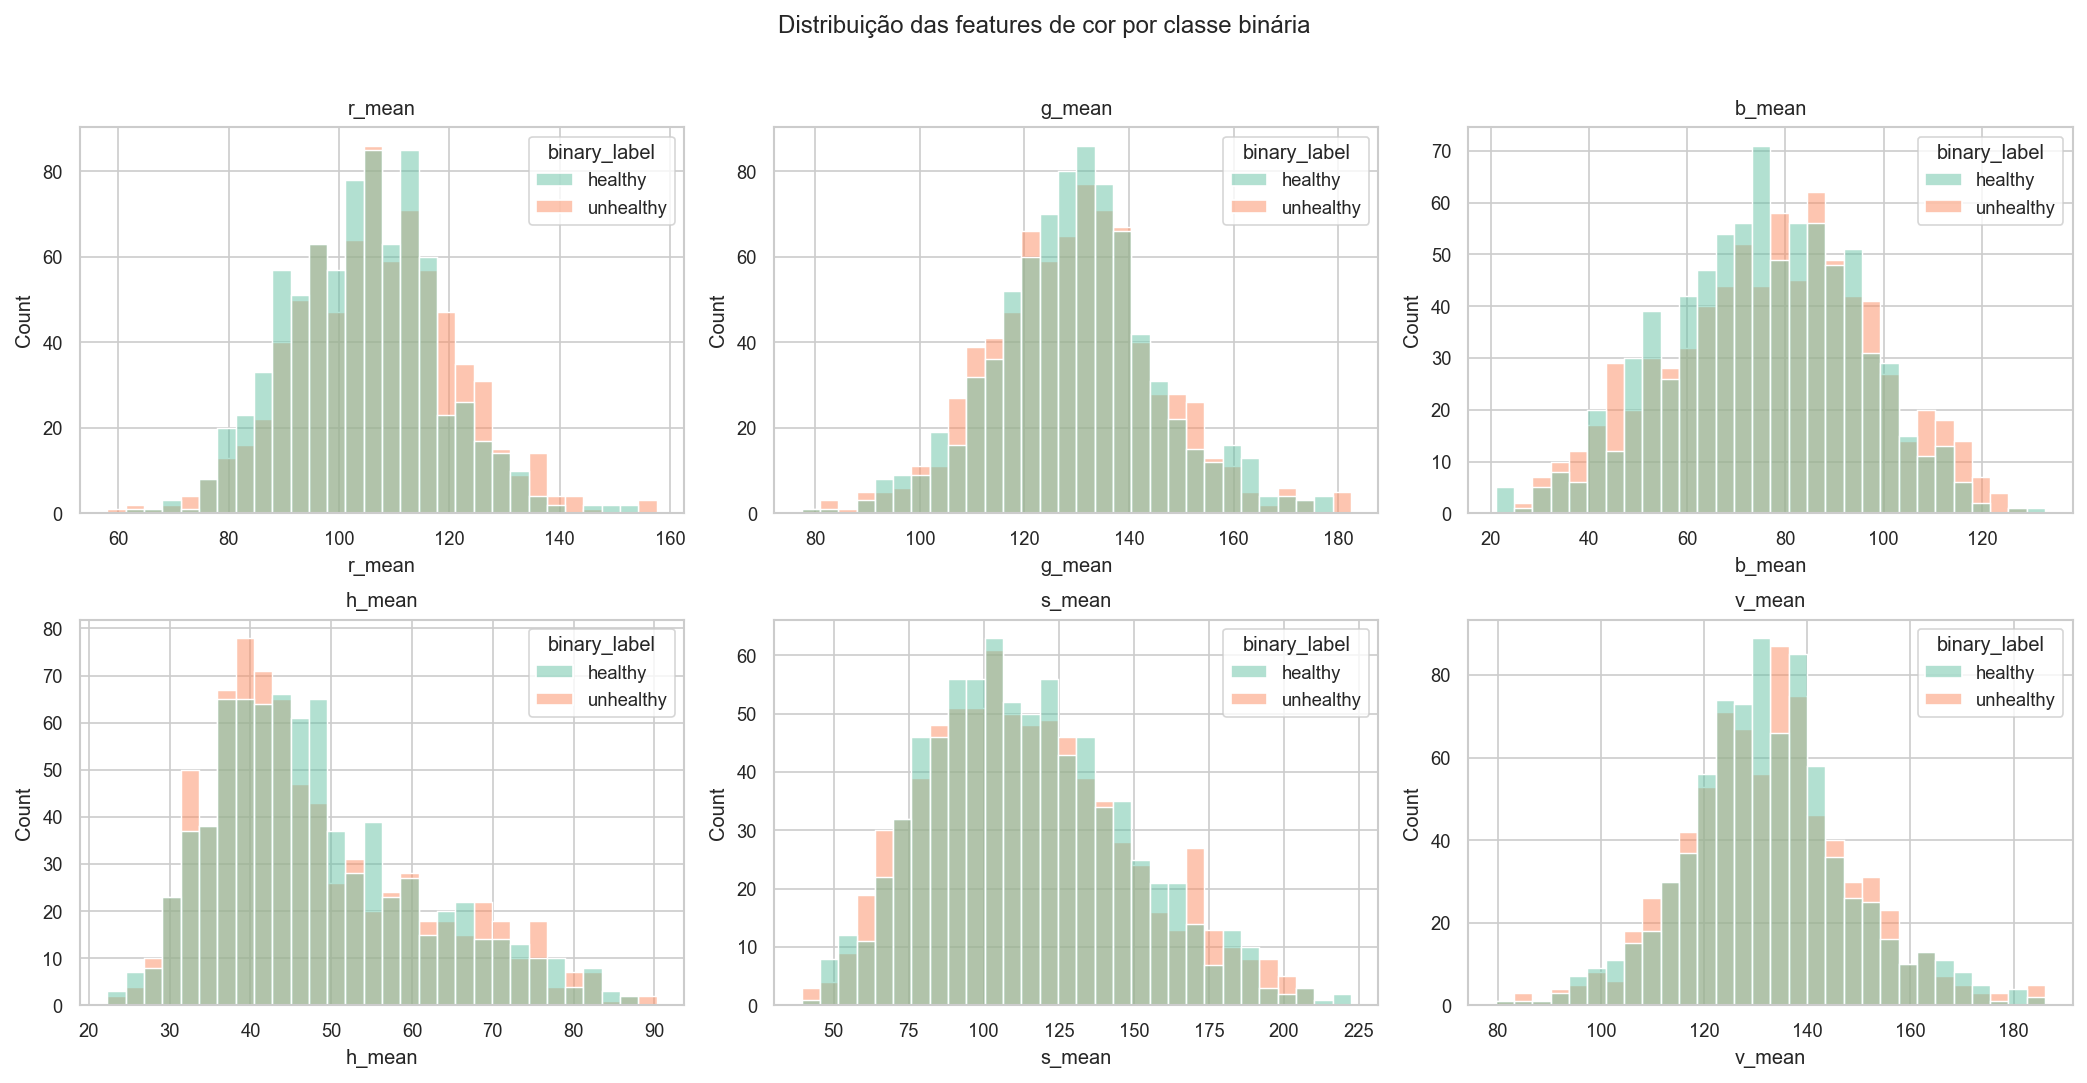
\includegraphics[width=\textwidth]{color_histograms.png}
\caption{Histogramas das \textit{features} médias de cor por classe binária.}
\label{fig:histcolor}
\end{figure}

\subsection{Boxplots das \textit{features}-chave por classe multiclasse}

A Figura~\ref{fig:boxplots} exibe \textit{boxplots} das nove \textit{features} mais informativas estratificados por classe multiclasse. As proporções cromáticas específicas por patologia revelam comportamentos distintos: a classe \textit{red\_spider\_mite} apresenta a maior mediana de \texttt{ratio\_rust\_brown\_orange} (0,050), consistente com a descoloração marrom-avermelhada típica da infestação. A classe \textit{rust\_level\_4} (severa) também se destaca (0,041), enquanto \textit{healthy} e \textit{rust\_level\_2} apresentam os menores valores medianos (0,022) --- provavelmente porque, em \textit{rust\_level\_2}, as lesões ainda são pontuais e não dominam a imagem.

\begin{figure}[H]
\centering
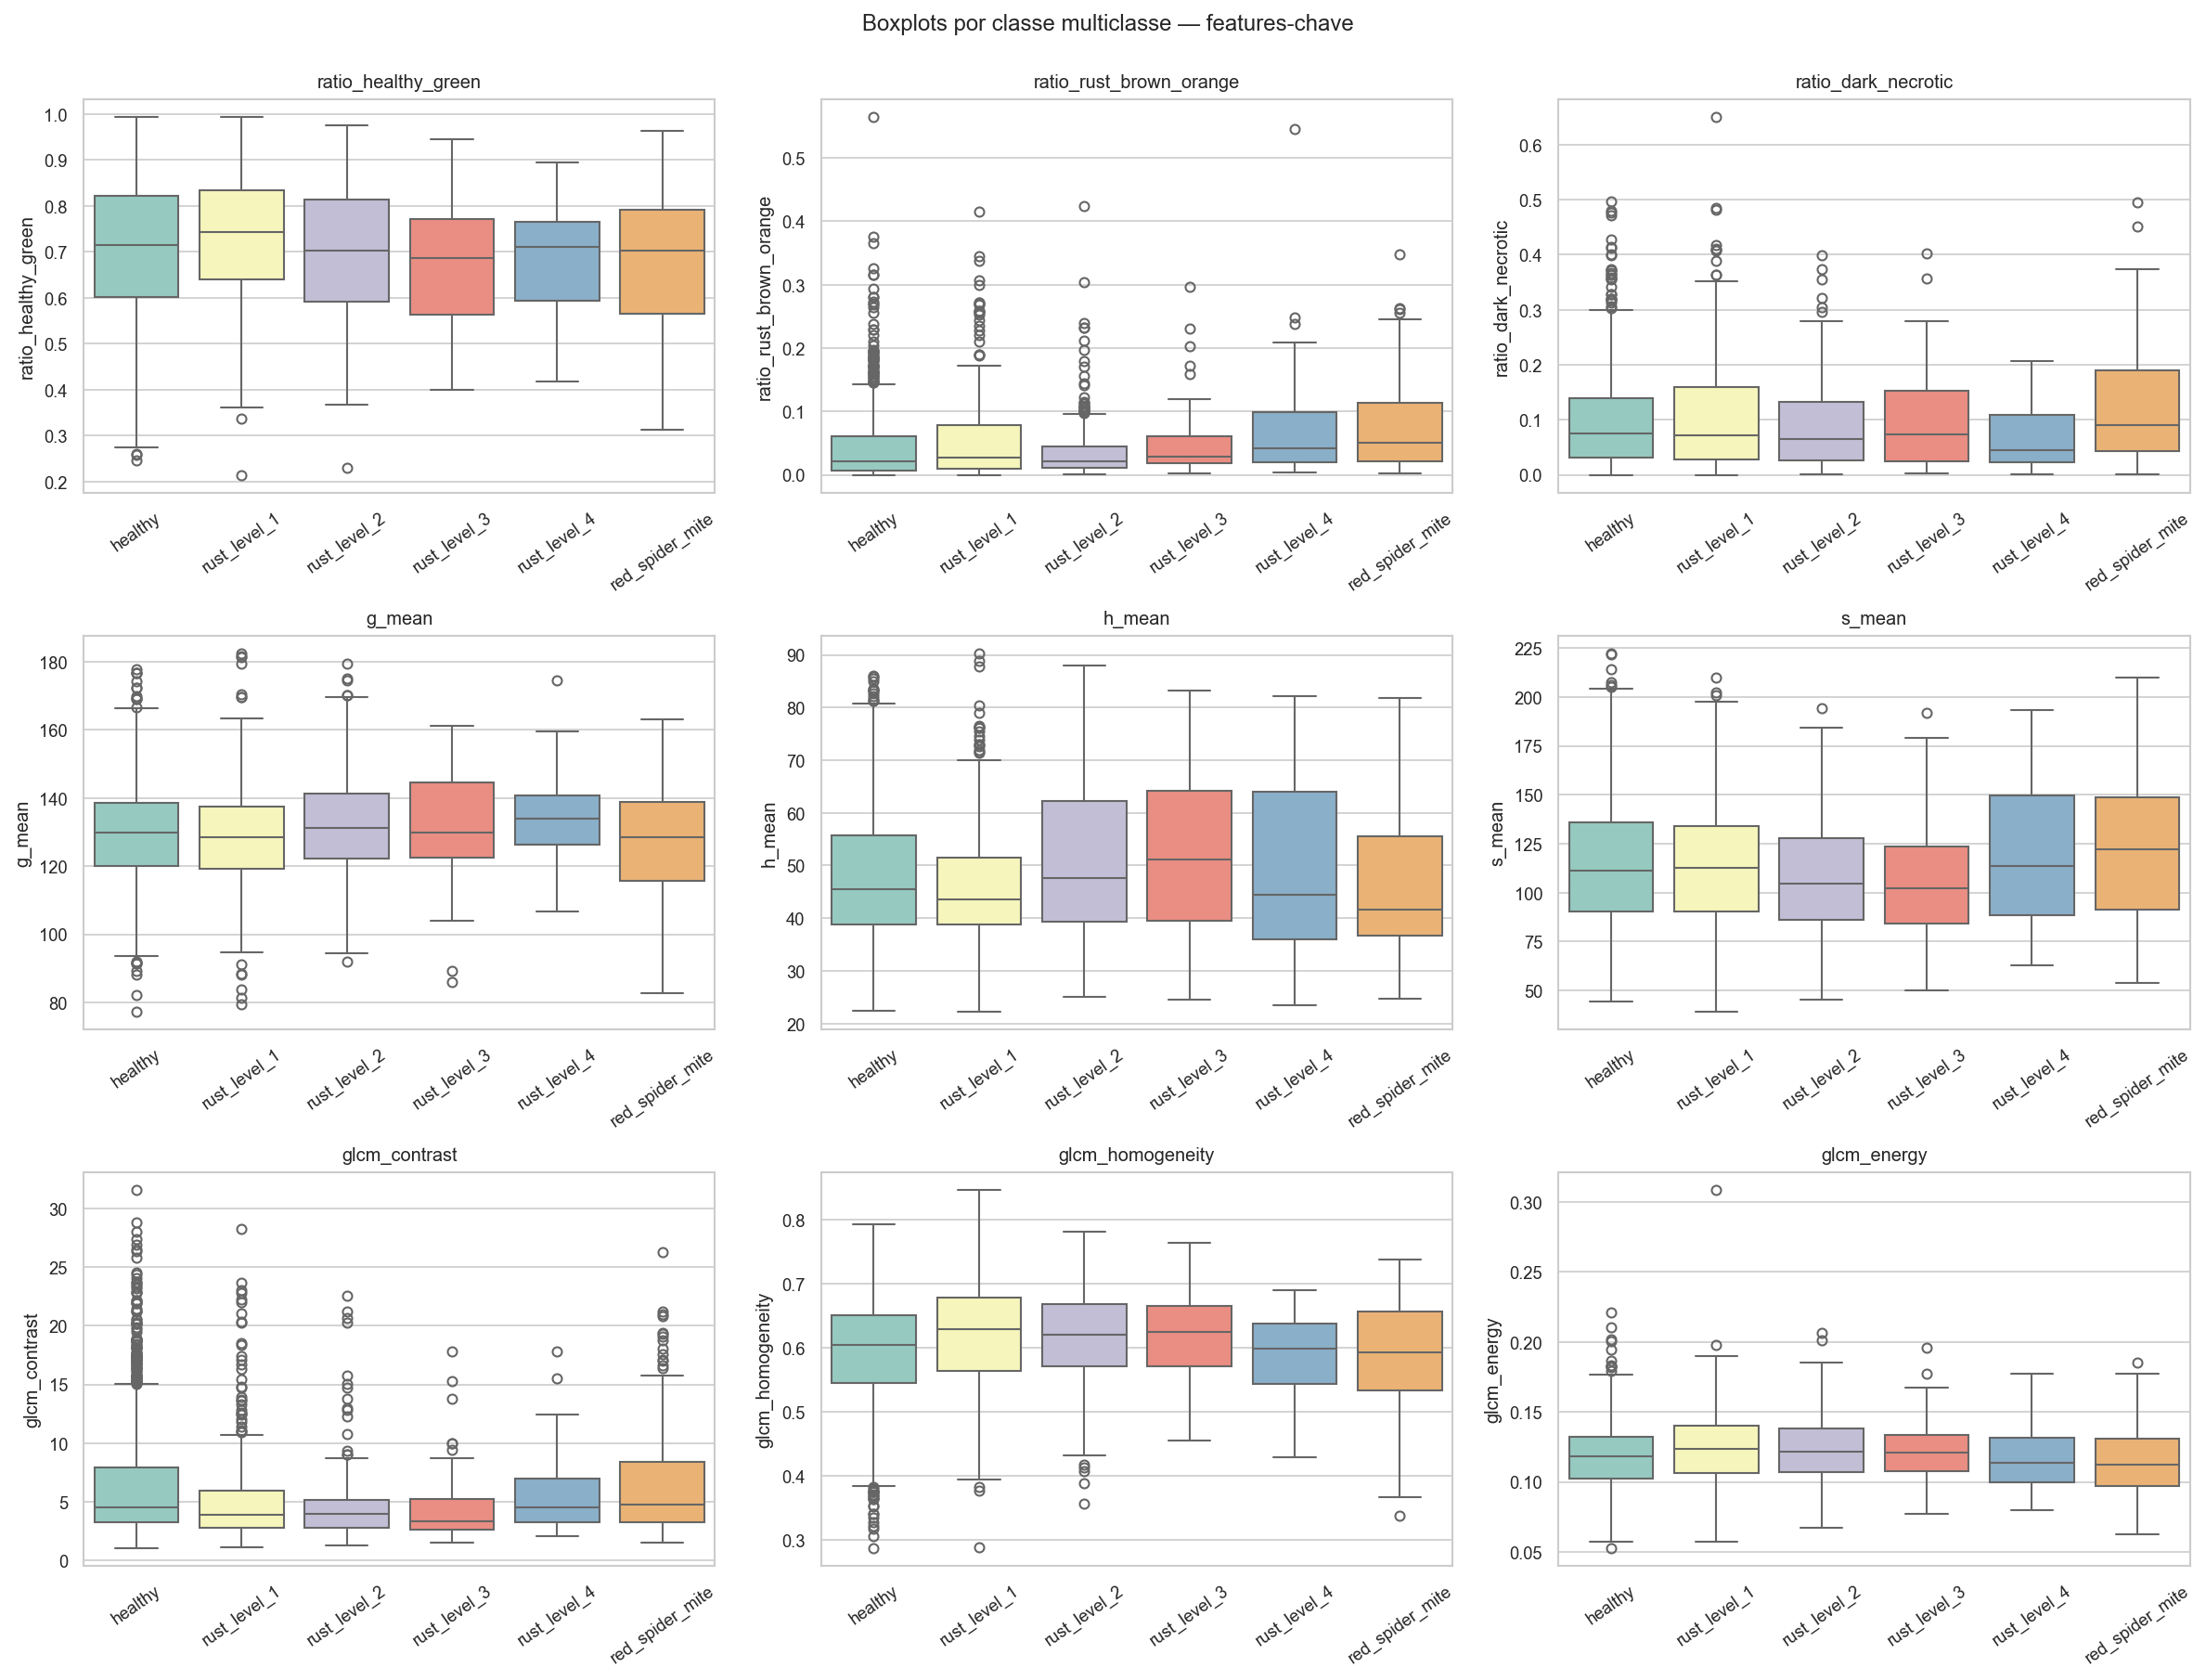
\includegraphics[width=\textwidth]{boxplots_keyfeats.png}
\caption{\textit{Boxplots} das \textit{features}-chave estratificados por classe multiclasse.}
\label{fig:boxplots}
\end{figure}

Um achado relevante é que \texttt{ratio\_healthy\_green} é \textit{maior} em \textit{rust\_level\_1} (0,743) do que em \textit{healthy} (0,714). Esse resultado contraintuitivo sugere que as imagens de folhas saudáveis podem ter sido capturadas com mais contexto de fundo (solo, galhos) do que as de folhas infectadas em estágio inicial, revelando um \textbf{viés sistemático de aquisição} que identifiquei como ponto crítico para a interpretação dos resultados.

\subsection{Matriz de correlação}

A Figura~\ref{fig:corr} apresenta a matriz de correlação de Pearson entre as 26 \textit{features}. Os cinco pares mais correlacionados (em valor absoluto) que observei são:

\begin{center}
\small
\begin{tabular}{ll r}
\toprule
\textbf{Feature A} & \textbf{Feature B} & $|r|$ \\
\midrule
\texttt{height} & \texttt{width} & 1{,}000 \\
\texttt{g\_std} & \texttt{v\_std} & 0{,}994 \\
\texttt{g\_mean} & \texttt{v\_mean} & 0{,}992 \\
\texttt{glcm\_contrast} & \texttt{laplacian\_var} & 0{,}982 \\
\texttt{glcm\_asm} & \texttt{glcm\_energy} & 0{,}981 \\
\bottomrule
\end{tabular}
\end{center}

\begin{figure}[H]
\centering
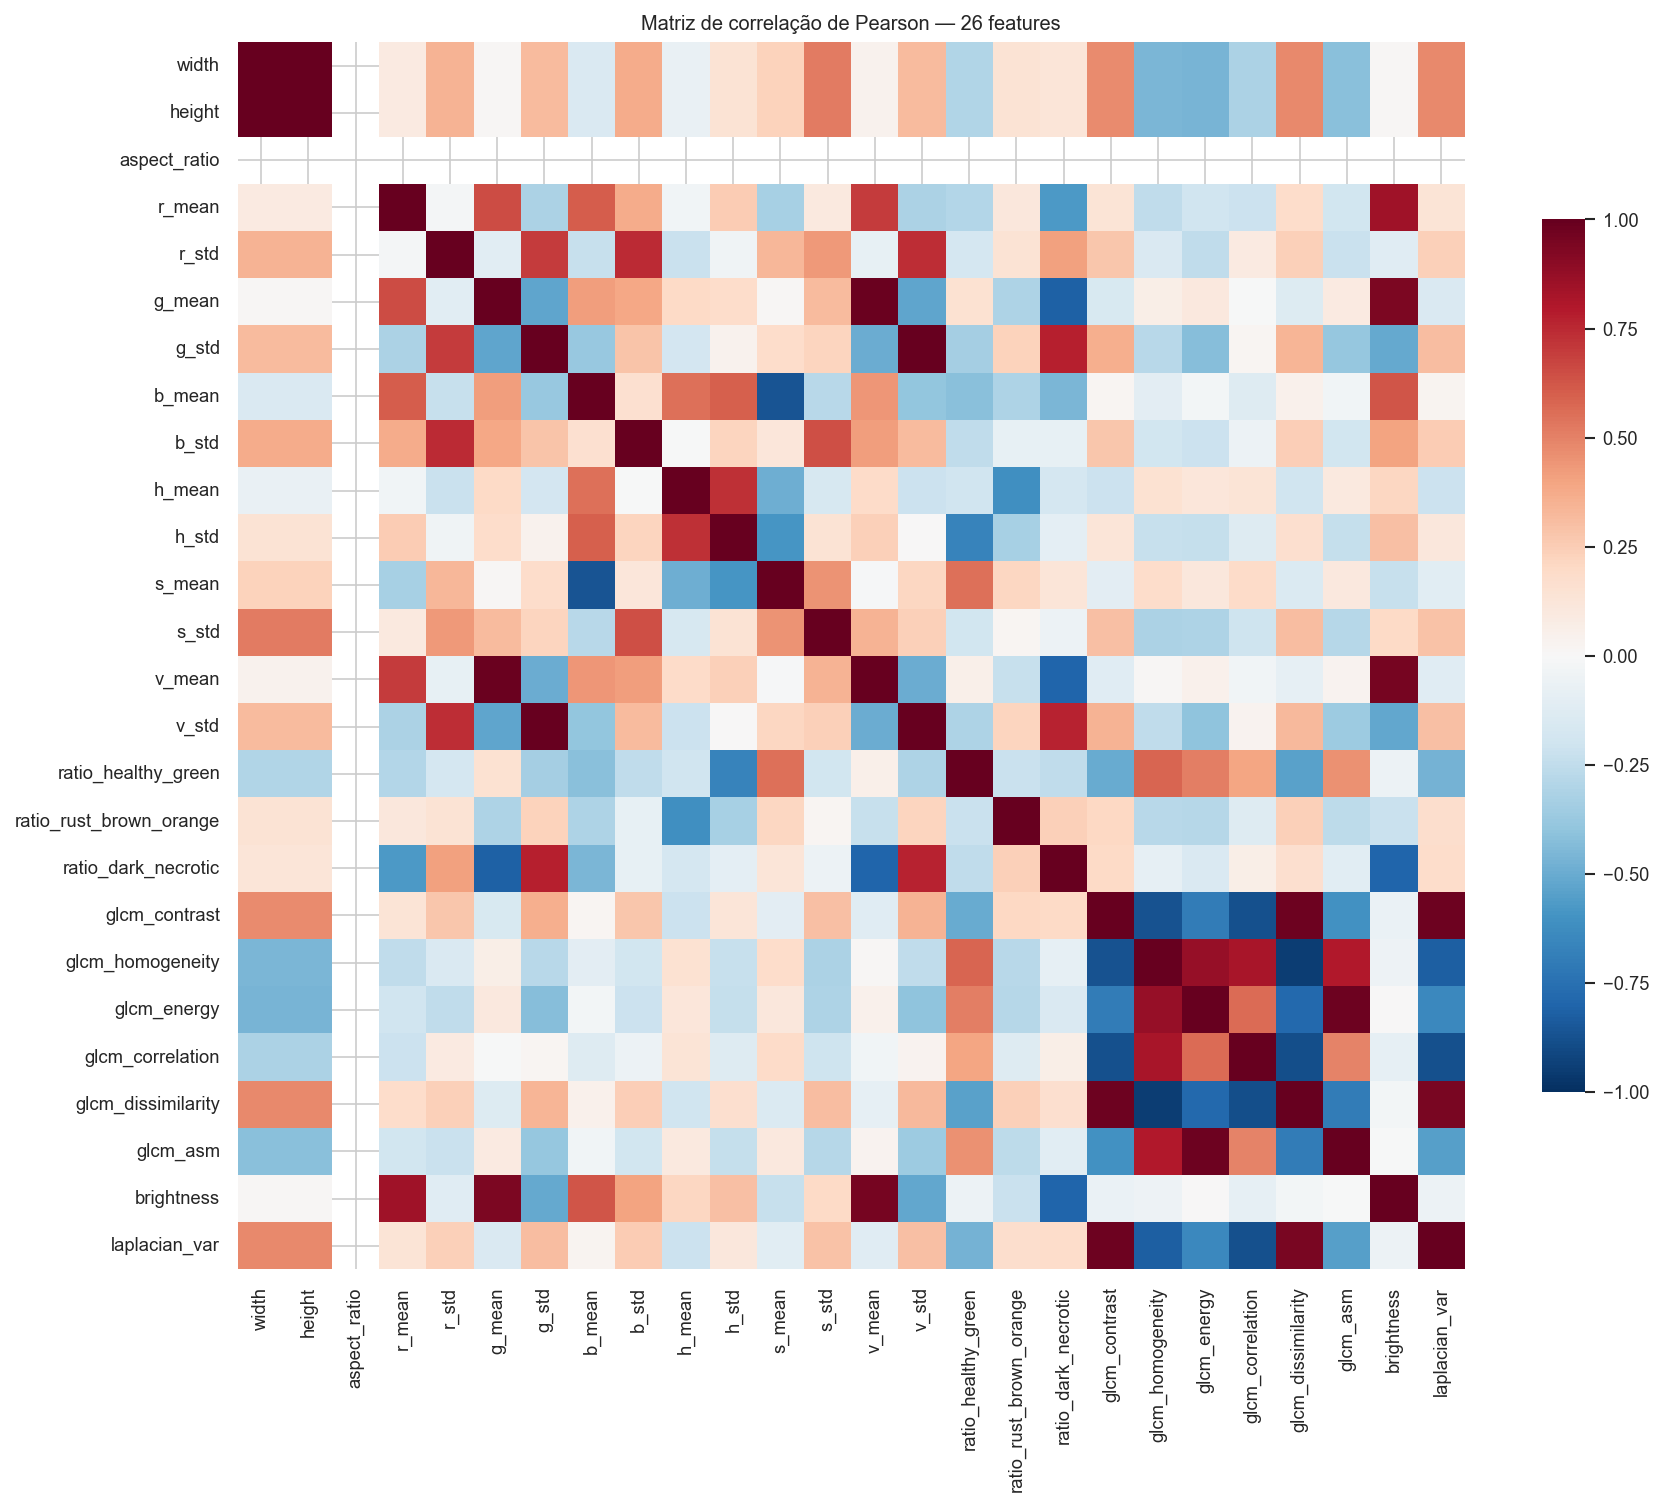
\includegraphics[width=0.80\textwidth]{correlation_matrix.png}
\caption{Matriz de correlação de Pearson entre as 26 \textit{features} tabulares.}
\label{fig:corr}
\end{figure}

A correlação perfeita entre \texttt{height} e \texttt{width} decorre da proporção fixa ($9{:}16$) de todas as imagens. As correlações elevadas entre canais G/V e entre \texttt{glcm\_asm} e \texttt{glcm\_energy} são matematicamente esperadas (o canal V do HSV é o máximo dos canais RGB em cada \textit{pixel}, e a energia GLCM é a raiz quadrada do ASM). Essa redundância entre \textit{features} é uma característica relevante a ser considerada em qualquer modelagem que use essas variáveis.

\subsection{Poder discriminativo das \textit{features} (ANOVA)}

A Figura~\ref{fig:anova} ordena as \textit{features} pelo F-\textit{score} da ANOVA em relação ao rótulo multiclasse. Os resultados revelam um \textbf{achado metodologicamente importante}: as dimensões (\texttt{width}, \texttt{height}) aparecem entre as \textit{features} mais discriminativas ($F=13{,}96$, $p < 10^{-12}$), superando descritores visuais como \texttt{glcm\_correlation} ($F=9{,}61$) e \texttt{laplacian\_var} ($F=8{,}91$).

\begin{figure}[H]
\centering
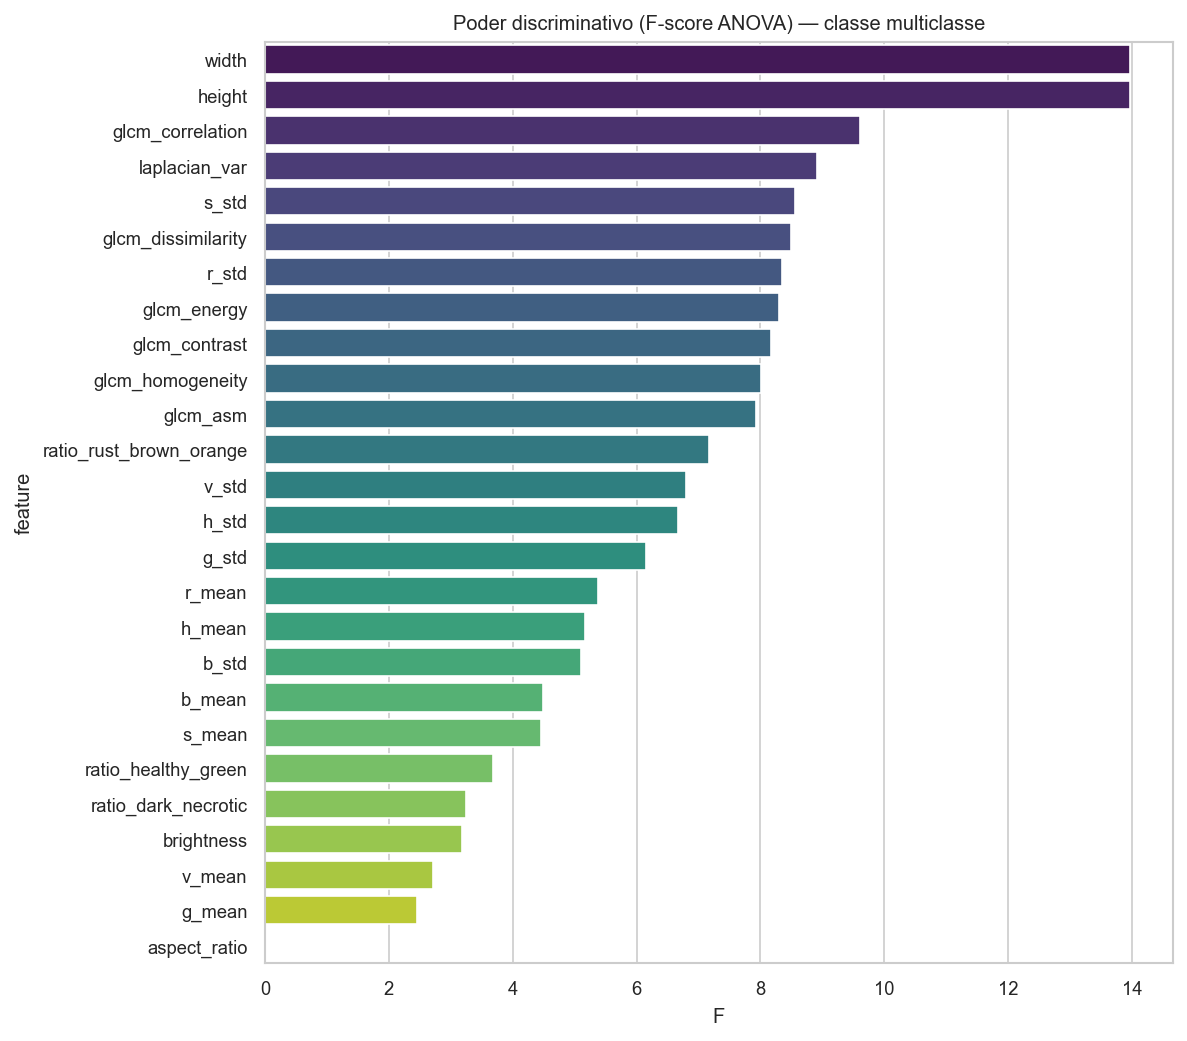
\includegraphics[width=0.90\textwidth]{anova_fscore.png}
\caption{Poder discriminativo (F-\textit{score} da ANOVA) de cada \textit{feature} em relação à classe multiclasse.}
\label{fig:anova}
\end{figure}

Interpreto esse resultado com cautela: ele não deve ser lido como valor preditivo legítimo. Ao contrário, revela que as condições de captura variaram sistematicamente entre classes, possivelmente porque diferentes sessões de campo (com dispositivos diferentes) documentaram patologias específicas. Trata-se de uma informação fundamental para a correta interpretação de qualquer classificador que venha a ser construído sobre este \textit{dataset}.

\subsection{Projeções em baixa dimensão}

A Figura~\ref{fig:proj} apresenta as projeções PCA e t-SNE do espaço de \textit{features} (após padronização). O PCA, capturando uma fração limitada da variância, mostra forte sobreposição entre classes. O t-SNE, por sua vez, revela uma estrutura local parcialmente coerente, com pequenos agrupamentos por classe, mas sem separação clara --- reforçando a expectativa de que classificadores lineares tenham desempenho limitado e que modelos não lineares (como \textit{Random Forest} e SVM com \textit{kernel} RBF) sejam mais adequados.

\begin{figure}[H]
\centering
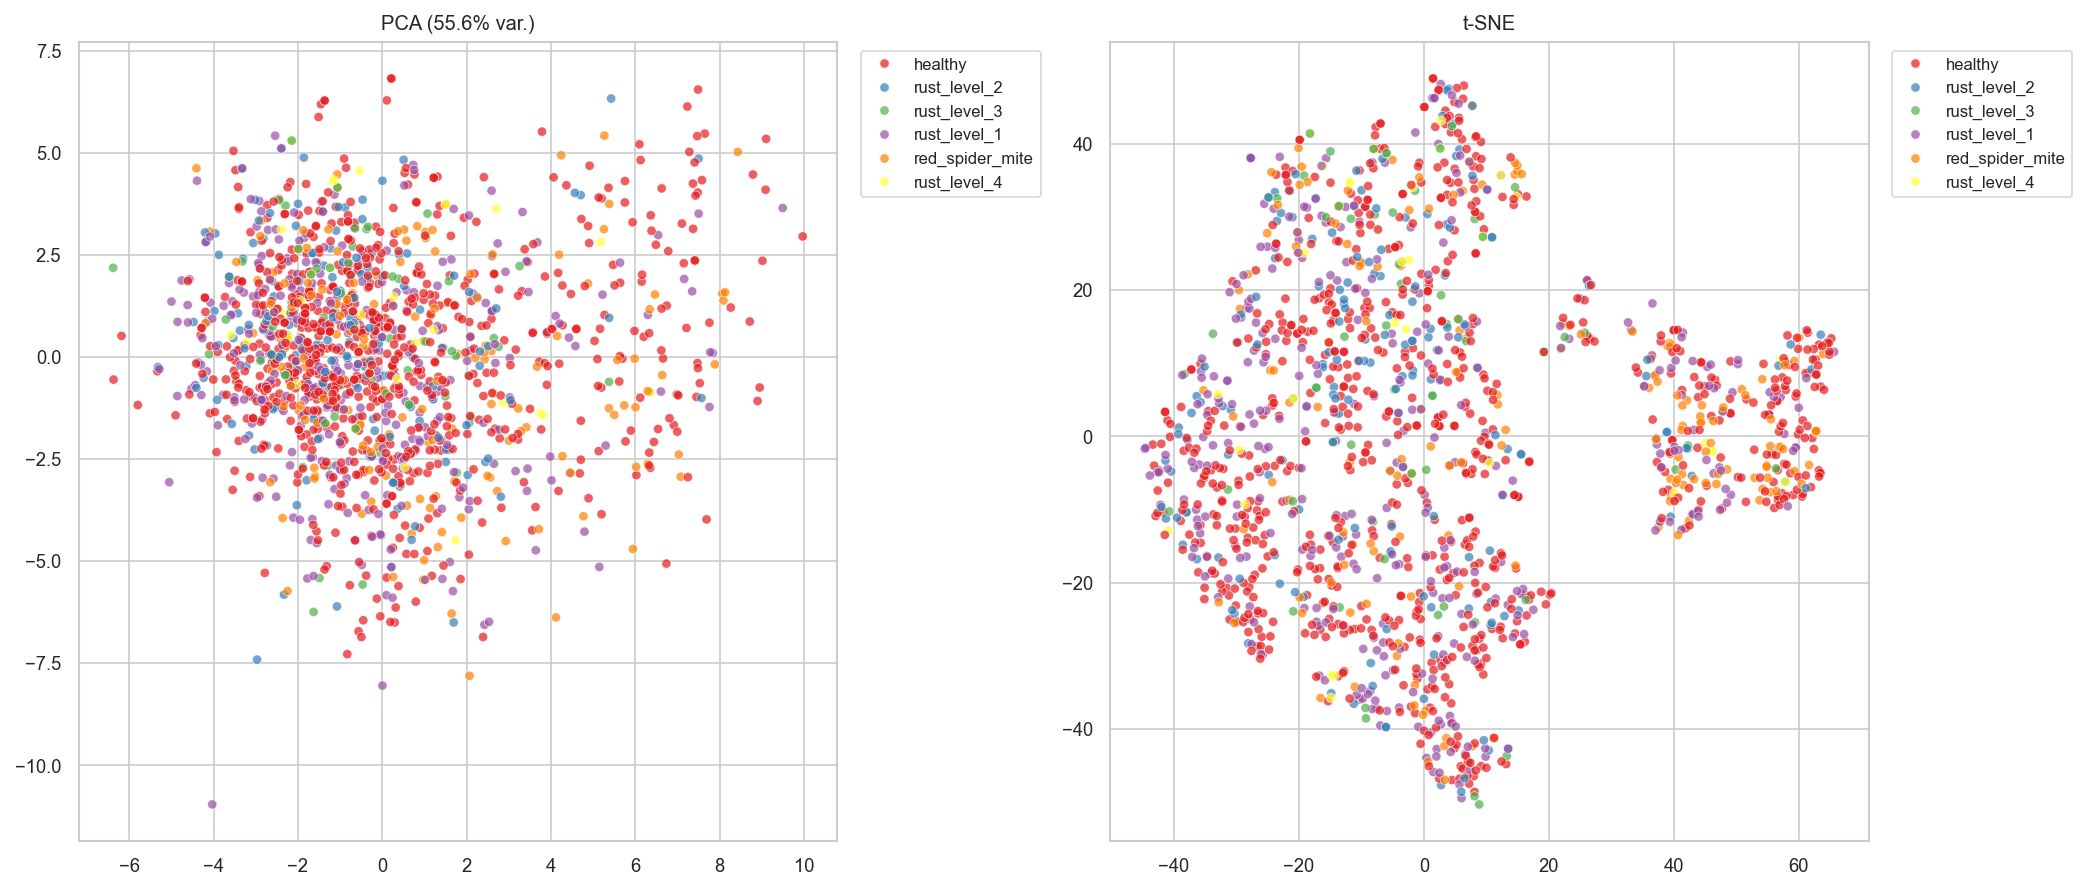
\includegraphics[width=\textwidth]{projections.png}
\caption{Projeções PCA (esquerda) e t-SNE (direita) do espaço de \textit{features}, coloridas pela classe multiclasse.}
\label{fig:proj}
\end{figure}

\subsection{Síntese dos \textit{insights}}

Consolido a seguir os principais achados da AED:

\begin{itemize}
  \item \textbf{Desbalanceamento multiclasse severo} (razão 26,4$\times$), característica que precisa ser contemplada em qualquer estratégia de avaliação.
  \item \textbf{Alta variabilidade de aquisição}, característica inerente de \textit{datasets} \textit{in situ} e desafio central para generalização.
  \item \textbf{Viés sistemático na captura}: dimensões de imagem correlacionam com classe; \textit{features} de cor média apresentam valores contraintuitivos entre classes.
  \item \textbf{Redundância entre \textit{features}}: existem pares com $|r| > 0{,}98$, indicando sobreposição informacional.
  \item \textbf{Sobreposição entre classes no espaço projetado}: as classes não se separam claramente em projeções lineares.
\end{itemize}

\section*{Disponibilização do Código}

O \textit{script} de extração de \textit{features} (\texttt{extract\_features.py}) e o \textit{notebook} Jupyter de AED (\texttt{aed\_rocole.ipynb}) acompanham este relatório e estão disponibilizados junto da entrega no Moodle.

\begin{thebibliography}{9}

\bibitem{conab}
Companhia Nacional de Abastecimento. \textit{Acompanhamento da safra brasileira de café}. 2024. Disponível em: \url{https://www.conab.gov.br}. Acesso em: jan. 2026.

\bibitem{matiello2016}
MATIELLO, J. B. et al. \textit{Cultura de café no Brasil: manual de recomendações}. 2. ed. Rio de Janeiro: MAPA/PROCAFÉ, 2016.

\bibitem{barbedo2018}
BARBEDO, J. G. A. Factors influencing the use of deep learning for plant disease recognition. \textit{Biosystems Engineering}, v. 172, p. 84--91, 2018.

\bibitem{barbedo2019}
BARBEDO, J. G. A. Plant disease identification from individual lesions and spots using deep learning. \textit{Biosystems Engineering}, v. 180, p. 96--107, 2019.

\bibitem{parraga2019}
PARRAGA-ALAVA, J.; CUSME, K.; LOOR, A.; SANTANDER, E. \textit{RoCoLe: A robusta coffee leaf images dataset}. Mendeley Data, v.2, 2019. DOI: 10.17632/c5yvn32dzg.2.

\bibitem{santos2023}
SANTOS, L. F. C.; OLIVEIRA, G. M. B.; SILVA, R. R. V. Classificação de doenças em folhas de café robusta utilizando redes neurais convolucionais. In: SBC, \textit{Anais do Workshop de Computação Aplicada à Gestão do Meio Ambiente e Recursos Naturais}. Porto Alegre, 2023. p. 61--70.

\bibitem{haralick1973}
HARALICK, R. M.; SHANMUGAM, K.; DINSTEIN, I. Textural features for image classification. \textit{IEEE Transactions on Systems, Man, and Cybernetics}, v. SMC-3, n. 6, p. 610--621, 1973.

\end{thebibliography}

\end{document}
